\documentclass[a4paper,12pt]{article}
\usepackage[utf8]{inputenc}
\usepackage[T1]{fontenc}
\usepackage{amsmath,amssymb}
\usepackage{tikz}
\usetikzlibrary{automata, positioning, arrows.meta}
\usepackage{booktabs}
\usepackage{array}
\usepackage{geometry}
\usepackage{listings}
\geometry{margin=0.9in}

\lstset{
  basicstyle=\ttfamily\small,
  frame=single,
  numbers=left,
  numberstyle=\tiny,
  breaklines=true,
  columns=fullflexible
}

\title{PLT 2026 --- Tutorial Week 3}
\author{}
\date{}

\begin{document}
\maketitle

%=============================================================
% GENERIC CODE (referenced throughout)
%=============================================================
\noindent\textbf{Generic Code} (used for all walkthroughs):

\begin{lstlisting}
state = initial_state;
cur_char = getchar();
while (true) {
    if (cur_char == EOI)
        break;
    next_state = T[state][cur_char];
    if (next_state == ERROR)
        state = next_state;
        break;
    state = next_state;
    cur_char = getchar();
}
if (is_final_state(state))
    return (valid_token);
else
    return (not_valid_token);
\end{lstlisting}

%=============================================================
% Q1: [0-9]*.[0-9]+
%=============================================================
\section{Question 1: \texttt{[0-9]*.[0-9]+}}

\subsection{DFSA}

\begin{center}
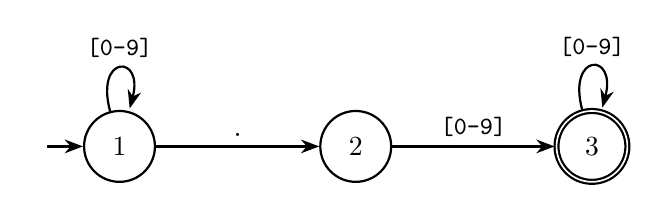
\begin{tikzpicture}[
    ->, >=Stealth, node distance=3cm,
    every state/.style={thick, minimum size=0.9cm},
    initial text={}, every edge/.style={draw, thick}, auto
]
    \node[state, initial]                (s1) {$1$};
    \node[state, right of=s1]           (s2) {$2$};
    \node[state, accepting, right of=s2] (s3) {$3$};

    \path
        (s1) edge[loop above]  node{\small\texttt{[0-9]}}  ()
        (s1) edge[above]       node{\small\texttt{.}}      (s2)
        (s2) edge[above]       node{\small\texttt{[0-9]}}  (s3)
        (s3) edge[loop above]  node{\small\texttt{[0-9]}}  ();
\end{tikzpicture}
\end{center}

State 1 = start (integer part);\;
State 2 = dot read;\;
State 3 = fractional part \textbf{(accept)}.

\subsection{Transition Table}

\begin{center}
\renewcommand{\arraystretch}{1.5}
\begin{tabular}{c|cc}
\toprule
\textbf{T} & \texttt{[0-9]} & \texttt{.} \\
\midrule
$\to$ \textbf{1} & T(1)  & T(2)  \\
\textbf{2}        & T(3)  & T(error) \\
\textbf{*3}       & T(3)  & T(error) \\
\bottomrule
\end{tabular}
\end{center}

\subsection{Walkthroughs}

\subsubsection*{Input: \texttt{.75}}

\begin{center}
\renewcommand{\arraystretch}{1.2}
\begin{tabular}{c|l|l|l}
\toprule
\textbf{Step} & \textbf{cur\_char} & \textbf{T[state][cur\_char]} & \textbf{state} \\
\midrule
init  & ---           & ---              & 1 \\
1     & \texttt{.}    & T[1][\texttt{.}] = 2     & 2 \\
2     & \texttt{7}    & T[2][\texttt{7}] = 3     & 3 \\
3     & \texttt{5}    & T[3][\texttt{5}] = 3     & 3 \\
4     & EOI           & break            & 3 \\
\bottomrule
\end{tabular}
\end{center}
\texttt{is\_final\_state(3)} = true $\Rightarrow$ \textbf{valid\_token}

\subsubsection*{Input: \texttt{86}}

\begin{center}
\renewcommand{\arraystretch}{1.2}
\begin{tabular}{c|l|l|l}
\toprule
\textbf{Step} & \textbf{cur\_char} & \textbf{T[state][cur\_char]} & \textbf{state} \\
\midrule
init  & ---           & ---              & 1 \\
1     & \texttt{8}    & T[1][\texttt{8}] = 1     & 1 \\
2     & \texttt{6}    & T[1][\texttt{6}] = 1     & 1 \\
3     & EOI           & break            & 1 \\
\bottomrule
\end{tabular}
\end{center}
\texttt{is\_final\_state(1)} = false $\Rightarrow$ \textbf{not\_valid\_token}

\subsubsection*{Input: \texttt{976.3}}

\begin{center}
\renewcommand{\arraystretch}{1.2}
\begin{tabular}{c|l|l|l}
\toprule
\textbf{Step} & \textbf{cur\_char} & \textbf{T[state][cur\_char]} & \textbf{state} \\
\midrule
init  & ---           & ---              & 1 \\
1     & \texttt{9}    & T[1][\texttt{9}] = 1     & 1 \\
2     & \texttt{7}    & T[1][\texttt{7}] = 1     & 1 \\
3     & \texttt{6}    & T[1][\texttt{6}] = 1     & 1 \\
4     & \texttt{.}    & T[1][\texttt{.}] = 2     & 2 \\
5     & \texttt{3}    & T[2][\texttt{3}] = 3     & 3 \\
6     & EOI           & break            & 3 \\
\bottomrule
\end{tabular}
\end{center}
\texttt{is\_final\_state(3)} = true $\Rightarrow$ \textbf{valid\_token}

%=============================================================
% Q2: [a-zA-Z][a-zA-Z0-9]*
%=============================================================
\newpage
\section{Question 2: \texttt{[a-zA-Z][a-zA-Z0-9]*}}

\subsection{DFSA}

\begin{center}
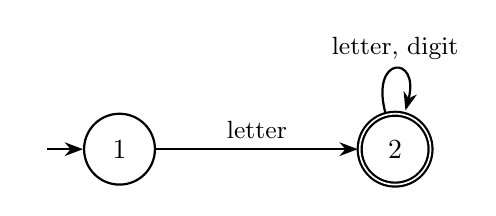
\begin{tikzpicture}[
    ->, >=Stealth, node distance=3.5cm,
    every state/.style={thick, minimum size=0.9cm},
    initial text={}, every edge/.style={draw, thick}, auto
]
    \node[state, initial]                (s1) {$1$};
    \node[state, accepting, right of=s1] (s2) {$2$};

    \path
        (s1) edge[above]       node{\small letter}          (s2)
        (s2) edge[loop above]  node{\small letter, digit}   ();
\end{tikzpicture}
\end{center}

State 1 = start;\;
State 2 = read at least one letter \textbf{(accept)}.

\subsection{Transition Table}

\begin{center}
\renewcommand{\arraystretch}{1.5}
\begin{tabular}{c|ccc}
\toprule
\textbf{T} & \textbf{letter} & \textbf{digit} & \textbf{other} \\
\midrule
$\to$ \textbf{1} & T(2)     & T(error) & T(error) \\
\textbf{*2}       & T(2)     & T(2)     & T(error) \\
\bottomrule
\end{tabular}
\end{center}

\subsection{Walkthroughs}

\subsubsection*{Input: \texttt{a92ad3}}

\begin{center}
\renewcommand{\arraystretch}{1.2}
\begin{tabular}{c|l|l|l}
\toprule
\textbf{Step} & \textbf{cur\_char} & \textbf{T[state][cur\_char]} & \textbf{state} \\
\midrule
init  & ---           & ---                       & 1 \\
1     & \texttt{a} (letter) & T[1][letter] = 2    & 2 \\
2     & \texttt{9} (digit)  & T[2][digit] = 2     & 2 \\
3     & \texttt{2} (digit)  & T[2][digit] = 2     & 2 \\
4     & \texttt{a} (letter) & T[2][letter] = 2    & 2 \\
5     & \texttt{d} (letter) & T[2][letter] = 2    & 2 \\
6     & \texttt{3} (digit)  & T[2][digit] = 2     & 2 \\
7     & EOI                 & break                & 2 \\
\bottomrule
\end{tabular}
\end{center}
\texttt{is\_final\_state(2)} = true $\Rightarrow$ \textbf{valid\_token}

\subsubsection*{Input: \texttt{3aty}}

\begin{center}
\renewcommand{\arraystretch}{1.2}
\begin{tabular}{c|l|l|l}
\toprule
\textbf{Step} & \textbf{cur\_char} & \textbf{T[state][cur\_char]} & \textbf{state} \\
\midrule
init  & ---               & ---                       & 1 \\
1     & \texttt{3} (digit) & T[1][digit] = ERROR      & ERROR \\
      &                    & break                     & \\
\bottomrule
\end{tabular}
\end{center}
\texttt{is\_final\_state(ERROR)} = false $\Rightarrow$ \textbf{not\_valid\_token}\\
(Starts with a digit, not a letter.)

\subsubsection*{Input: \texttt{ty5\^{}}}

\begin{center}
\renewcommand{\arraystretch}{1.2}
\begin{tabular}{c|l|l|l}
\toprule
\textbf{Step} & \textbf{cur\_char} & \textbf{T[state][cur\_char]} & \textbf{state} \\
\midrule
init  & ---                & ---                       & 1 \\
1     & \texttt{t} (letter) & T[1][letter] = 2         & 2 \\
2     & \texttt{y} (letter) & T[2][letter] = 2         & 2 \\
3     & \texttt{5} (digit)  & T[2][digit] = 2          & 2 \\
4     & \texttt{\^{}} (other) & T[2][other] = ERROR    & ERROR \\
      &                     & break                     & \\
\bottomrule
\end{tabular}
\end{center}
\texttt{is\_final\_state(ERROR)} = false $\Rightarrow$ \textbf{not\_valid\_token}\\
(\texttt{\^{}} is not a letter or digit.)

%=============================================================
% Q3: C variable regex
%=============================================================
\newpage
\section{Question 3: FLEX Regex for C Variable}

\noindent\textbf{Rules:}
\begin{itemize}
  \item Unlimited-length sequence of letters, digits, and underscores
  \item Must \emph{not} begin with a digit
  \item If it begins with \texttt{\_}, that must be followed by a letter,
        then unlimited letters/digits/underscores
\end{itemize}

\noindent\textbf{Examples:} \texttt{g},\; \texttt{e17},\; \texttt{\_ty},\;
\texttt{r\_u\_ready},\; \texttt{\_t}.

% ---- Solution A ----
\subsection{Solution A --- Alternation (\texttt{|})}

\begin{center}
\large
\texttt{[a-zA-Z][a-zA-Z0-9\_]*|\_[a-zA-Z][a-zA-Z0-9\_]*}
\end{center}

Two alternatives joined by \texttt{|}: the left branch starts with a letter,
the right branch starts with \texttt{\_} followed by a required letter.
Both then allow unlimited continuation characters.

\begin{center}
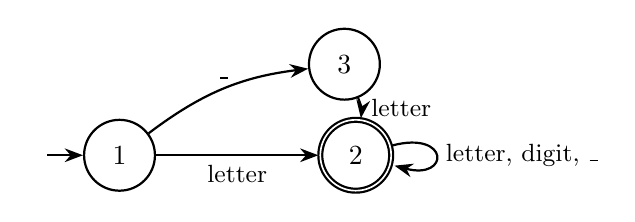
\begin{tikzpicture}[
    ->, >=Stealth, node distance=3cm,
    every state/.style={thick, minimum size=0.9cm},
    initial text={}, every edge/.style={draw, thick}, auto
]
    \node[state, initial]                         (s1) {$1$};
    \node[state, accepting, right of=s1]          (s2) {$2$};
    \node[state, above right=0.5cm and 2.2cm of s1] (s3) {$3$};

    \path
        (s1) edge[below]              node{\small letter}                     (s2)
        (s1) edge[above, bend left=15] node{\small \texttt{\_}}              (s3)
        (s3) edge[right, bend left=15] node{\small letter}                   (s2)
        (s2) edge[loop right]          node{\small letter, digit, \texttt{\_}} ();
\end{tikzpicture}
\end{center}

% ---- Solution B ----
\subsection{Solution B --- Optional (\texttt{?})}

\begin{center}
\large
\texttt{\_?[a-zA-Z][a-zA-Z0-9\_]*}
\end{center}

\texttt{\_?} means zero or one underscore. After the optional underscore a
letter is always required, then unlimited continuation. More concise
than Solution~A but describes the same language.

\begin{center}
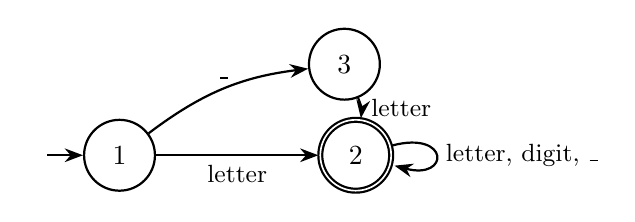
\begin{tikzpicture}[
    ->, >=Stealth, node distance=3cm,
    every state/.style={thick, minimum size=0.9cm},
    initial text={}, every edge/.style={draw, thick}, auto
]
    \node[state, initial]                         (s1) {$1$};
    \node[state, accepting, right of=s1]          (s2) {$2$};
    \node[state, above right=0.5cm and 2.2cm of s1] (s3) {$3$};

    \path
        (s1) edge[below]              node{\small letter}                     (s2)
        (s1) edge[above, bend left=15] node{\small \texttt{\_}}              (s3)
        (s3) edge[right, bend left=15] node{\small letter}                   (s2)
        (s2) edge[loop right]          node{\small letter, digit, \texttt{\_}} ();
\end{tikzpicture}
\end{center}

% ---- Solution C ----
\subsection{Solution C --- Grouped alternation}

\begin{center}
\large
\texttt{([a-zA-Z]|\_[a-zA-Z])[a-zA-Z0-9\_]*}
\end{center}

The opening group handles both start cases (plain letter \emph{or}
underscore-then-letter), then a single shared continuation
\texttt{[a-zA-Z0-9\_]*} follows.

\begin{center}
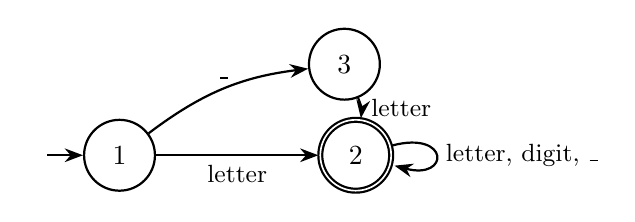
\begin{tikzpicture}[
    ->, >=Stealth, node distance=3cm,
    every state/.style={thick, minimum size=0.9cm},
    initial text={}, every edge/.style={draw, thick}, auto
]
    \node[state, initial]                         (s1) {$1$};
    \node[state, accepting, right of=s1]          (s2) {$2$};
    \node[state, above right=0.5cm and 2.2cm of s1] (s3) {$3$};

    \path
        (s1) edge[below]              node{\small letter}                     (s2)
        (s1) edge[above, bend left=15] node{\small \texttt{\_}}              (s3)
        (s3) edge[right, bend left=15] node{\small letter}                   (s2)
        (s2) edge[loop right]          node{\small letter, digit, \texttt{\_}} ();
\end{tikzpicture}
\end{center}

\medskip\noindent
\textbf{Note:} All three regular expressions describe the \emph{same}
language, so they produce the \emph{same} minimal DFSA (3~states).
The difference is purely syntactic---\texttt{|} (alternation),
\texttt{?} (zero-or-one), and grouping \texttt{()} are three ways to
express the optional leading underscore.

% ---- Verification ----
\subsection{Verification Against Examples}

\begin{center}
\renewcommand{\arraystretch}{1.3}
\begin{tabular}{llll}
\toprule
\textbf{String} & \textbf{A} & \textbf{B} & \textbf{C} \\
\midrule
\texttt{g}            & Yes & Yes & Yes \\
\texttt{e17}          & Yes & Yes & Yes \\
\texttt{\_ty}         & Yes & Yes & Yes \\
\texttt{r\_u\_ready}  & Yes & Yes & Yes \\
\texttt{\_t}          & Yes & Yes & Yes \\
\texttt{\_\_x} (invalid) & No & No & No \\
\texttt{3ab}  (invalid) & No & No & No \\
\bottomrule
\end{tabular}
\end{center}

%=============================================================
% Q4: DFSA for C variable
%=============================================================
\newpage
\section{Question 4: DFSA for C Variable Token}

\subsection{DFSA}

(Same automaton for all three regex solutions above.)

\begin{center}
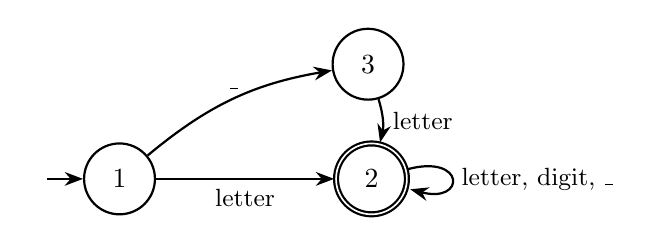
\begin{tikzpicture}[
    ->, >=Stealth, node distance=3.2cm,
    every state/.style={thick, minimum size=0.9cm},
    initial text={}, every edge/.style={draw, thick}, auto
]
    \node[state, initial]                         (s1) {$1$};
    \node[state, accepting, right of=s1]          (s2) {$2$};
    \node[state, above right=0.8cm and 2.5cm of s1] (s3) {$3$};

    \path
        (s1) edge[below]              node{\small letter}                     (s2)
        (s1) edge[above, bend left=15] node{\small \texttt{\_}}              (s3)
        (s3) edge[right, bend left=15] node{\small letter}                   (s2)
        (s2) edge[loop right]          node{\small letter, digit, \texttt{\_}} ();
\end{tikzpicture}
\end{center}

State 1 = start;\;
State 2 = valid identifier body \textbf{(accept)};\;
State 3 = read leading underscore, need a letter.

\subsection{Transition Table}

\begin{center}
\renewcommand{\arraystretch}{1.5}
\begin{tabular}{c|cccc}
\toprule
\textbf{T} & \textbf{letter} & \textbf{digit} & \texttt{\_} & \textbf{other} \\
\midrule
$\to$ \textbf{1} & T(2)     & T(error) & T(3)     & T(error) \\
\textbf{*2}       & T(2)     & T(2)     & T(2)     & T(error) \\
\textbf{3}        & T(2)     & T(error) & T(error) & T(error) \\
\bottomrule
\end{tabular}
\end{center}

%=============================================================
% Q5: Walk through Ay65__ and H67$%
%=============================================================
\section{Question 5: Walkthroughs for C Variable Token}

\subsection*{Input: \texttt{Ay65\_\_}}

\begin{center}
\renewcommand{\arraystretch}{1.2}
\begin{tabular}{c|l|l|l}
\toprule
\textbf{Step} & \textbf{cur\_char} & \textbf{T[state][cur\_char]} & \textbf{state} \\
\midrule
init  & ---                       & ---                        & 1 \\
1     & \texttt{A} (letter)       & T[1][letter] = 2           & 2 \\
2     & \texttt{y} (letter)       & T[2][letter] = 2           & 2 \\
3     & \texttt{6} (digit)        & T[2][digit] = 2            & 2 \\
4     & \texttt{5} (digit)        & T[2][digit] = 2            & 2 \\
5     & \texttt{\_} (underscore)  & T[2][\texttt{\_}] = 2      & 2 \\
6     & \texttt{\_} (underscore)  & T[2][\texttt{\_}] = 2      & 2 \\
7     & EOI                       & break                       & 2 \\
\bottomrule
\end{tabular}
\end{center}
\texttt{is\_final\_state(2)} = true $\Rightarrow$ \textbf{valid\_token}

\subsection*{Input: \texttt{H67\$\%}}

\begin{center}
\renewcommand{\arraystretch}{1.2}
\begin{tabular}{c|l|l|l}
\toprule
\textbf{Step} & \textbf{cur\_char} & \textbf{T[state][cur\_char]} & \textbf{state} \\
\midrule
init  & ---                     & ---                        & 1 \\
1     & \texttt{H} (letter)     & T[1][letter] = 2           & 2 \\
2     & \texttt{6} (digit)      & T[2][digit] = 2            & 2 \\
3     & \texttt{7} (digit)      & T[2][digit] = 2            & 2 \\
4     & \texttt{\$} (other)     & T[2][other] = ERROR        & ERROR \\
      &                         & break                       & \\
\bottomrule
\end{tabular}
\end{center}
\texttt{is\_final\_state(ERROR)} = false $\Rightarrow$ \textbf{not\_valid\_token}\\
(\texttt{\$} is not a letter, digit, or underscore.)

\end{document}
